\NEW{
\section{\newname: Real-time and Dynamic Bandwidth Separation with Online Traffic}
\label{sec:dynamic}

\begin{figure}[t]
  \centering
  %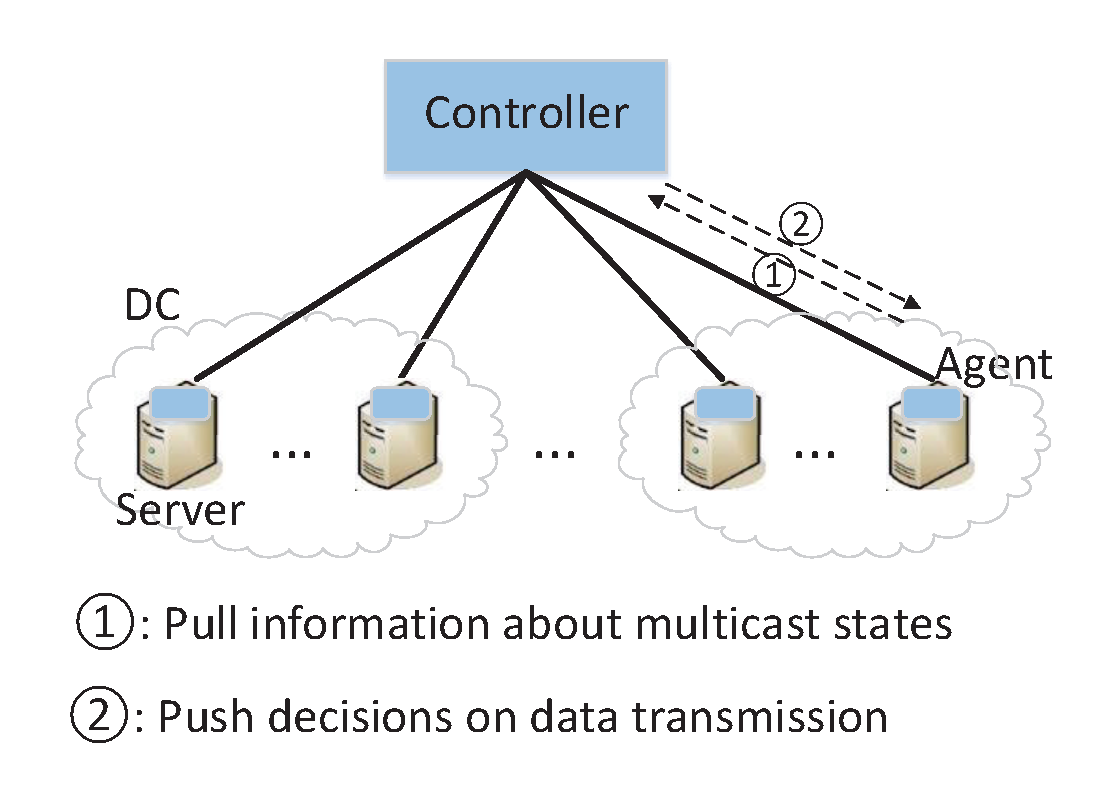
\includegraphics[width=2in]{images/framework.eps}
  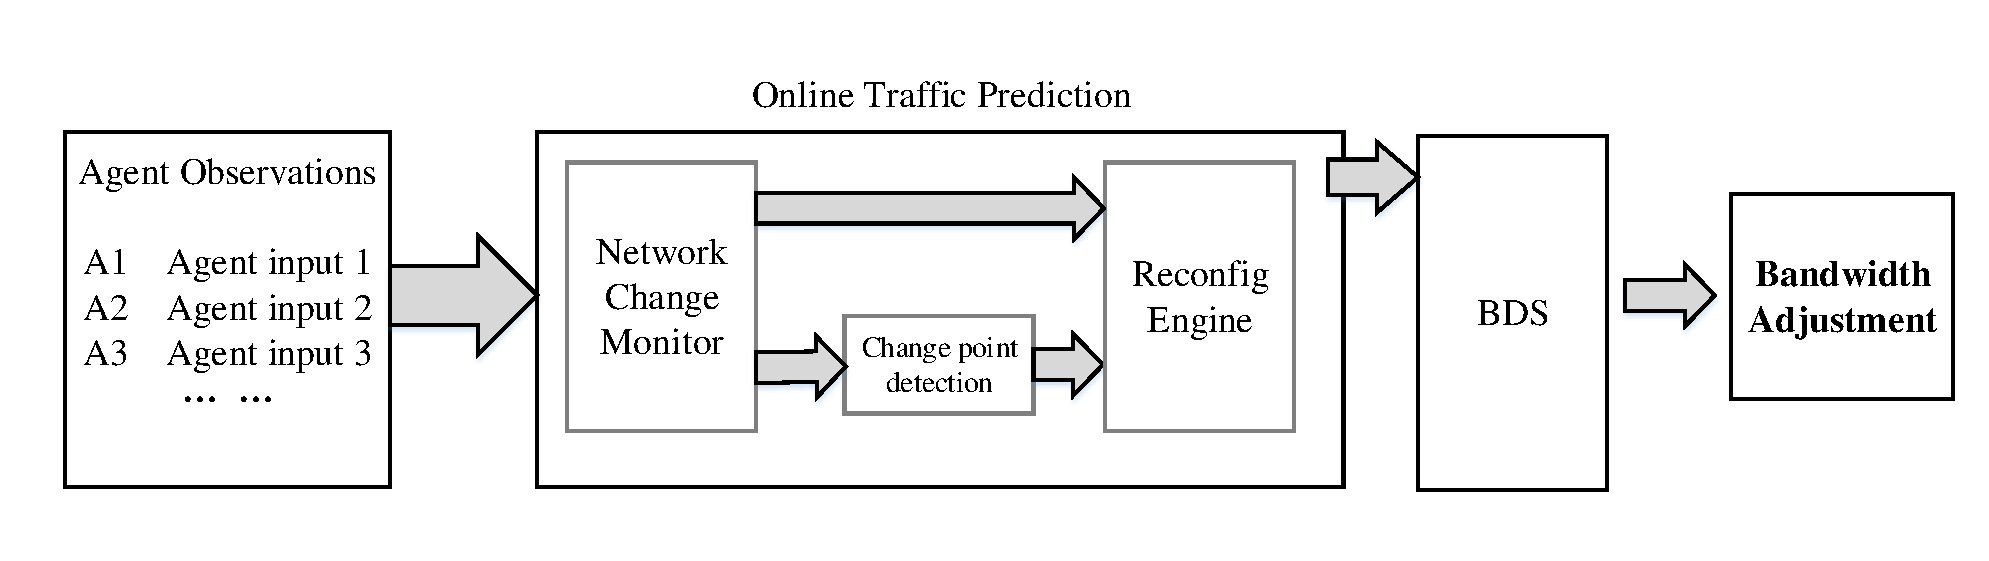
\includegraphics[width=3.4in]{images/Bayes.pdf}
    \vspace{-0.2cm}
  \tightcaption{\NEW{Logical diagram of \newname's online prediction.}}
  \label{fig:bayes}
\vspace{-0.4cm}
\end{figure}

\name performs well under strict network limitations, but sometimes results in bandwidth under-utilization. This is because the static \name bandwidth allocation algorithm {\em has limited dynamic range}: it will not occupy a greater bandwidth even when online traffic is in a valley, as there is a strict safety threshold for bulk data transfer to avoid excessive link utilization (\Section\ref{subsec:motivation:baseline}).

In this section, we present an enhanced version of \name, called \newname. \newname achieves dynamic bandwidth separation from online traffic in a real-time manner by continuously predicting online traffic changes and automatically adjusting the scheduling decisions to fully utilize network bandwidth. Thus, \newname automatically adjusts the scheduling results under different network conditions: if online traffic is at a peak, \newname shirk reduces its bandwidth to avoid congestion, while when online traffic is in a valley, \newname  aggressively uses more bandwidth to fully utilize network.

To achieve the above aim, \newname uses an online traffic prediction algorithm, which identifies if the bandwidth utilization of servers has changed significantly, and consequently signaling a bandwidth adjustment if it is needed. \newname's Network Change Monitor (Figure~\ref{fig:bayes}) observes bandwidth usage reported by the agents  and implements a change point detection algorithm. The Reconfig Engine is responsible for updating the changes based on agent observations and the detection results, reporting the changes to the \name controller and enforcing the subsequent bandwidth adjustment.

\subsection{Online traffic prediction}
\label{subsec:dynamic:prediction}
\mypara{Approaches to detect online traffic changes}
In order to detect online traffic changes and adjust configurations in time series, there are two widely adopted approaches: a change point detection algorithm, or an exponentially weighted moving average (EWMA) control scheme. A change point detection algorithm identifies sudden changes in sequential data and can be implemented in either an online of offline form. Offline methods \cite{smith1975bayesian,stephens1994bayesian,barry1993bayesian,green1995reversible} require the complete time series data to generate detection from the posterior distribution over change point locations. Online methods \cite{page1955test,desobry2005online,lorden1971procedures} can generate an accurate distribution of the next unseen data with only already observed data. An EWMA control scheme \cite{roberts1959control,lucas1990exponentially} calculates the mean and standard deviation of agent observations. However, EWMA based control can result in continual reconfiguration even when the network is (statistically) stationary since network traffic has naturally occurring variation.

\mypara{Change point detection algorithms}
\newname chooses an onlin change point detection algorithm \cite{adams2007bayesian} to predict traffic for two reasons. First, the agent of \name generates a sequence of observations per cycle, which is naturally non-overlapping states that are independent and identically distributed. This aligns well with the way change point detection algorithms works. Second, such algorithms require no \emph{a priori} knowledge, matching our scenario where we re-calculate the bulk multicast overlay routing problem periodically. For the BDS+ Network Change Monitor we implemented the algorithm introduced by \cite{adams2007bayesian} using available code \cite{BOCDcode}).

\mypara{Detecting online traffic changes}
During a scheduling cycle $\Delta T_k$ in \name, the Network Change Monitor is continually fed with server bandwidth usage observations from the agents, which is used to detect online traffic changes. The change point detection algorithm calculates the standard deviation of server throughput by only considering the samples in recent state history. To determine the bandwidth usage, the Network Change Monitor periodically reads the relevant record in the process activity monitor on servers to generate fine-grained samples (at milliseconds level). As servers already continuously log process activities (including throughput), sampling the summed throughput does not incur any additional overhead, and the only addition is to pass these samples to the Network Change Monitor. In this way, any fine-grained online traffic changes occurring during the bulk data downloading can be detected.


\subsection{Fine-granularity adjustments}
\label{subsec:dynamic:incremental}
When a change in the online traffic is detected, the Reconfig Engine signals the change and the updated available bandwidth to the Controller, enabling bandwidth adjustments in \newname to better utilize the ever-changing network. As shown in Table~\ref{table:adjustment}, such an adjustment is two-fold in nature (assuming the affected path by the online traffic change is $\hat{P}$):

\begin{table}[t]
\begin{center}
\resizebox{3in}{!}{
%\begin{tabular}{p{2cm}<{\centering}|p{2cm}<{\centering}}
\begin{tabular}{| c | c| c|}
\hline
 \rowcolor[gray]{0.9}
\textbf{Changes/Adjustments} & \textbf{Scheduling} &  \textbf{Routing} \\
\hline \hline
Online Traffic $\uparrow$ & $w^{(T_k)}_{b,s}$ - & $f_{b,p\in \hat{P}}^{(T_k)} \downarrow$\\
\hline
Online Traffic $\downarrow$ & $w^{(T_k)}_{b,s}$ + & $f_{b,p\in \hat{P}}^{(T_k)} \uparrow$\\
\hline
\end{tabular}
}
\end{center}
\tightcaption{\NEW{Real time adjustment in \newname according to the detected online traffic changes.}}
\label{table:adjustment}
\vspace{-0.4cm}
\end{table}

\begin{packeditemize}
\item When online traffic usage exceeds the pre-configured safety threshold (80\% in the example in \Section\ref{subsec:motivation:baseline}), \newname can make corrections on both scheduling and routing steps: 1. cancel some blocks that were scheduled in the current scheduling cycle $\Delta T$ but not yet transferred; 2. reduce the allocated bandwidth $f_{b,p}^{(T_k)}$ for block $b$ on path $p\in \hat{P}$ in $T_k$, to reduce bandwidth usage.

\item When online traffic usage falls below that threshold, \newname can also make corrections on both scheduling and routing steps: 1. transfer some additional blocks that were not scheduled in the current scheduling cycle $\Delta T$ by using the detected available bandwidth; 2. increase the allocated bandwidth $f_{b,p}^{(T_k)}$ for block $b$ on path $p\in \hat{P}$ in $T_k$, to make full use of the residual bandwidth detected by the online traffic prediction.
\end{packeditemize}

\mypara{Achieving low computational overhead}
Such fine-grained adjustments pose a significant challenge for the centralized controller, i.e., the online traffic prediction is executed in real-time, and thus requires the controller to update the decisions in the order of milliseconds. Although \name already decouples the scheduling and routing step to reduce the algorithm running time to hundreds of milliseconds, it is still not practical to update detection and adjustments in real time.

To address this challenge, \newname further optimizes the centralized algorithm by pruning the unaffected links from the optimisation space, \emph{i.e.} those links where there is no online traffic change detected. In other words, the fine-grained adjustments are only conducted on those servers/links that have increasing or decreasing available bandwidth, noting that the online traffic is relatively stationary over the millisecond level. Thus, most servers/links can be removed from the optimization space, and corresponding fine-grained adjustments can then be implemented in a very lightweight way with quite low computational overhead.

}
